\chapter{Experience Cannot Be Googled}

This interview segment turns on a simple question: how do sales skills become useful in company ownership? The answer does not begin with financing, structure, or management theory. It begins with field experience. Sales matters here because it forces repeated contact with refusal, and it trains the person to keep the same attitude while still delivering the message clearly.

\section{From Salesman To Company Owner}

The opening question asks how the skills learned from being a salesman helped someone own a company at a young age. That is the local problem of the passage. We should not smooth it into a general claim that sales is useful. The speaker is asked for a transfer: what carries over from selling into owning?

His answer is deliberately concrete. He does not begin with a technique. He begins with the statement that experience cannot be searched for and possessed. It must be gone through.

\subsection{Question \& Answer}

\paragraph{Question.}
How do sales skills translate into company ownership?

\paragraph{Answer.}
They translate because sales puts a person under live commercial pressure. A script, a polished appearance, and good advice may prepare the surface, but the deeper skill comes from being rejected repeatedly and still delivering the message in the right way.

That is the hinge of the whole passage. Sales does not automatically make a person an owner. It trains a behavior that ownership later needs: communicating clearly when the other side is not giving easy approval.

\section{Experience Versus Information}

The first distinction is between information and experience. Information can be searched, watched, copied, and rehearsed. Experience, in the speaker's usage, is not like that. It is the accumulation of actual encounters: cold calls, door knocking, angry responses, repeated refusal, and conversations with people who do not all hear the same message in the same way.

\begin{definition}
In this chapter, \emph{sales experience} means lived exposure to prospects, rejection, and varied conversations, not merely knowledge of sales language or technique.
\end{definition}

This distinction is the speaker's first move because it blocks the easy shortcut. A person can learn phrases, memorize a pitch, and look the part, but none of that proves that the person can still function when the answer is no. Entrepreneurship inherits the same test. The market does not only test what we know; it tests whether we can keep acting coherently under resistance.

\section{Surface Preparation And Field Skill}

The speaker is careful not to reject preparation. Someone can teach tricks, useful things to say, and even how to dress. Those are real forms of preparation. But they remain incomplete until they are tested against live response.

\begin{table}
\centering
\begin{tabular}{p{0.42\linewidth}p{0.42\linewidth}}
\hline
Surface preparation & Field-tested skill \\
\hline
Things to say & Saying them after rejection \\
Dressing well & Staying composed under pressure \\
Sales tricks & Adjusting to a real person \\
Instruction & Repetition through live encounters \\
\hline
\end{tabular}
\caption{The passage contrasts teachable preparation with the field pressure that turns preparation into usable sales ability.}
\end{table}

The order matters. The answer first grants that preparation exists, then shows its limit. A person has not yet learned the deeper skill until the pitch has survived refusal, anger, and repetition.

\section{Rejection As The Training Medium}

The passage then sharpens. The speaker lists the conditions that make sales formative: being told no, being cussed out, being screamed at, and hearing no after no after no. This is not a decorative list. It is the environment in which the skill is formed.

\begin{definition}
\emph{Rejection pressure} is repeated refusal or hostility from prospects while the salesperson remains responsible for delivering the message clearly.
\end{definition}

The useful lesson is not simply that rejection is unpleasant. The useful lesson is that rejection changes the conditions under which communication happens. If every refusal changes the salesperson's attitude, tone, or clarity, then the message deteriorates. Sales exposes that deterioration quickly.

\section{The Same Attitude}

The speaker's central mechanism appears in the phrase that one must still have the same attitude and still be able to deliver the message the right way. This is where rejection becomes training rather than merely suffering.

\begin{figure}
\centering
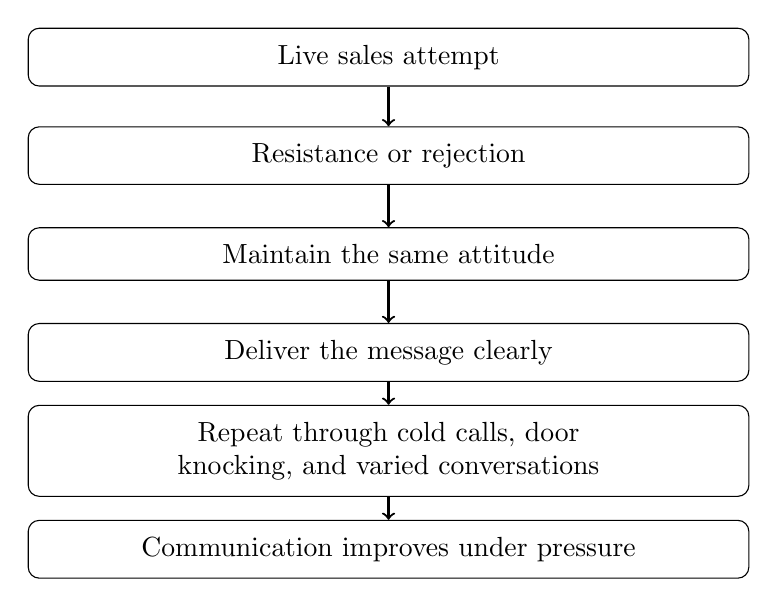
\begin{tikzpicture}[
  every node/.style={
    draw,
    rounded corners,
    align=center,
    text width=0.72\linewidth,
    inner sep=6pt
  },
  arrow/.style={->, thick}
]
\node (a) at (0,0) {Live sales attempt};
\node (b) at (0,-1.25) {Resistance or rejection};
\node (c) at (0,-2.50) {Maintain the same attitude};
\node (d) at (0,-3.75) {Deliver the message clearly};
\node (e) at (0,-5.00) {Repeat through cold calls, door knocking, and varied conversations};
\node (f) at (0,-6.25) {Communication improves under pressure};

\draw[arrow] (a) -- (b);
\draw[arrow] (b) -- (c);
\draw[arrow] (c) -- (d);
\draw[arrow] (d) -- (e);
\draw[arrow] (e) -- (f);
\end{tikzpicture}
\caption{A transcript-derived process view of the speaker's argument. The figure is a reconstruction of the spoken sequence, not an on-screen diagram.}
\end{figure}

This is the closest thing in the passage to a mechanism. The result is not produced by attitude alone, and not by repetition alone. It is produced by repeated attempts in which the person is forced to preserve the message after resistance has arrived.

\section{Thousands Of Repetitions}

The speaker then returns to the first claim in a stronger form. There is no textbook substitute, he says, except making thousands and thousands of cold calls, knocking on doors, and going through many different experiences.

We should preserve the phrase ``thousands and thousands'' as a qualitative magnitude, not as a measured statistic. The point is volume under variation. Each encounter repeats the sales task, but the person on the other side changes: the mood changes, the objection changes, the patience changes, and the background changes.

\begin{remark}
The claim is not that books, scripts, or coaching have no value. The claim is that they cannot substitute for enough live encounters to make the behavior durable.
\end{remark}

This is where the answer begins to point back toward company ownership. An owner must repeatedly represent an offer to customers, employees, vendors, partners, and sometimes investors. Not every one of those conversations is a sales call, but many require the same underlying discipline: keep the message clear while the situation pushes back.

\section{Communication Across Difference}

The final movement widens the lesson. Sales teaches communication with different types of people: different ethnicities, backgrounds, ages, and experiences. The speaker's claim is therefore broader than rejection tolerance. Sales also trains range.

A narrow social setting can reward a narrow style of communication. Sales does not. It forces the salesperson to notice that the same words may not land the same way with every person. The work becomes a practical education in how different people hear, resist, question, and decide.

\begin{proposition}
In the speaker's account, sales contributes to company ownership by training adaptable communication under repeated rejection and social variety.
\end{proposition}

\begin{proof}
The argument unfolds in order. First, the speaker distinguishes lived experience from searchable information. Second, he acknowledges teachable surface preparation but says it remains incomplete until tested. Third, he identifies repeated rejection as the test. Fourth, he names the required behavior: maintain the same attitude and deliver the message properly. Fifth, he grounds that behavior in thousands of cold calls, door knocking, and many experiences. Finally, he broadens the setting to communication across different backgrounds, ages, and experiences. Taken together, these steps support the proposition: sales trains the kind of communication that remains usable under pressure and across difference.
\end{proof}

\section{Summary}

The passage answers an entrepreneurial question by refusing the shortcut. Sales helped because it supplied experience that could not be Googled: cold calls, door knocking, rejection, and conversations with many kinds of people. The valuable skill was not merely knowing what to say. It was keeping the same attitude and delivering the message correctly after resistance. In this interview, sales becomes a bridge to ownership because it trains clear communication when the market is not cooperating.